\documentclass[11pt,letterpaper]{article}
\usepackage[margin=0.85in]{geometry}
\usepackage[T1]{fontenc}
\usepackage{lmodern}
\usepackage{amsmath,amssymb}
\usepackage{booktabs,longtable,array}
\usepackage{graphicx}
\usepackage[hidelinks]{hyperref}
\usepackage{url}
\setlength{\parskip}{0.35em}
\setlength{\parindent}{0pt}
\setlength{\emergencystretch}{2em}
\newcommand{\code}[1]{\texttt{\detokenize{#1}}}
\title{Decision Tree Induction for Classification\\
\large Implementation, Correctness Validation, and Comparison on Ten Benchmarks}
% Fill in the assignment-information fields below before submitting.
\author{Pei Ma\\[0.4em]\large ESE 327: Fundamental Algorithms in Machine Learning Systems}
\date{November 22, 2026}

\begin{document}
\maketitle

\begin{abstract}
A binary decision-tree classifier was implemented in Python and NumPy
using three split criteria: information gain, gain ratio, and Gini impurity reduction. 
The custom implementation was compared with logistic regression, five-nearest 
neighbors, and Gaussian naive Bayes classification algorithms on ten prepared 
benchmark datasets.  
Each of the 60 dataset--model
configurations was run in a fresh process three times, producing 180 measured
runs. 
Validation combines hand-calculated examples, 20 automated tests, and an
audit of every saved run against its predictions and source data.
Five-nearest neighbors achieved the highest average accuracy and macro-averaged
F1 score, while logistic regression offered similar accuracy with substantially
faster prediction.
\end{abstract}

\tableofcontents
\clearpage

\section{Objective and implementation scope}
The objective is to implement decision-tree induction for classification,
experiment with three split criteria, and compare the resulting classifier with
three other classification algorithms. Information gain, gain ratio,
and Gini impurity reduction are configurations of the same custom tree implementation; they are
not counted as the three additional algorithms. The additional methods are
logistic regression, five-nearest neighbors, and Gaussian naive Bayes, 
using scikit-learn implementations.

The tree's node representation, exact threshold search, recursive construction,
and prediction traversal were implemented in this project. NumPy supplies array
operations; no library decision-tree training routine is called. All algorithms
receive the same saved training and test partitions.

The experiment results reported here come exclusively from
\code{results/comparison/}, not the earlier tree-only pilot results. The trees
were rerun alongside the baselines with the same import, threading, batching,
and measurement policy. Twenty tests and the saved-results audit passed when
preparing this report.

\section{Decision-tree induction algorithm}
\subsection{Representation and prediction}
Each node stores its training-sample count and majority-class prediction.
An internal node additionally stores a feature index $j$, threshold $t$, and
left/right children. A row follows the left branch when $x_j\leq t$ and the
right branch otherwise. A leaf returns its majority class. Original labels are
mapped to consecutive integers during training and mapped back for prediction.
Class-count ties choose the first sorted class, making the outcome reproducible.

The processed input is numeric. Categorical features have already been expanded
into binary one-hot columns. Thus, a categorical indicator is split like any
other numeric feature, generally at $0.5$. This is a binary threshold tree,
not a native multiway categorical tree. Although the criteria are standard
decision-tree quantities, the implementation is not a complete
reproduction of an established tree-learning system: it has no post-pruning,
and its gain-ratio configuration uses the ratio directly without additional
candidate-selection safeguards.

\subsection{How the split criteria choose a branch}
A split criterion measures how well a proposed split separates the classes.
A useful split creates child groups with clearer class membership than the
parent group. All three options examine the same candidate thresholds; only
the scoring rule changes.

\begin{description}
\item[Information gain.] Entropy describes how mixed the class labels are
within a group. It is zero when every example belongs to the same class and
increases when the labels are more evenly mixed. Information gain measures how
much a split reduces that uncertainty. The tree chooses the split with the
largest reduction, accounting for the number of examples in each child.
\item[Gain ratio.] Gain ratio starts with information gain and adjusts it
using a quantity called split information, which depends on how examples are
distributed between the two branches. This changes the relative scores of
balanced and uneven splits. A high ratio does not necessarily mean the largest
absolute reduction in uncertainty, so the implementation also requires a
positive information gain before accepting a split.
\item[Gini impurity reduction.] Gini impurity is another measure of class mixing: it is
zero for a group containing only one class and larger for a mixed group.
The tree compares the parent's impurity with the combined impurity of its two
children, weighted by their sizes, and chooses the largest decrease.
\end{description}

These criteria offer different ways to rank a split, rather than different
training pipelines. The experiment keeps preprocessing, candidate thresholds,
and stopping rules the same so that their effects can be compared directly.
The worked example in Section~\ref{sec:realexample} shows how these scores
are calculated from a few training rows.

\subsection{Exact candidate search}
At each node, the algorithm sorts each feature and considers thresholds
between distinct adjacent values. Cumulative class counts let it score all
candidates efficiently. It rejects splits that leave fewer than two rows in
a child or fail to reduce impurity, then selects the highest-scoring candidate.
Ties follow a fixed feature and threshold order. Thresholds use midpoints,
with a floating-point safeguard to keep adjacent values on the correct sides.

\subsection{Construction and stopping rules}
The following is the actual \code{_build} method from
\code{algorithms/decision_tree.py}. It creates a majority-class node, checks
whether splitting should stop, and otherwise recursively builds its children.

\begingroup\scriptsize
\begin{verbatim}
def _build(self, indices, depth):
    """Recursively partition rows until a stopping condition produces a leaf."""
    counts = np.bincount(self._y[indices], minlength=len(self.classes_))
    
    node = Node(prediction=int(np.argmax(counts)), samples=len(indices))
    self.node_count_ += 1
    self.depth_ = max(self.depth_, depth)
    stop = (np.count_nonzero(counts) == 1 or
            len(indices) < max(self.min_samples_split, 2 * self.min_samples_leaf) or
            (self.max_depth is not None and depth >= self.max_depth))
    split = None if stop else self._best_split(indices, counts)
    
    if split is None:
        self.leaf_count_ += 1
        return node
    node.feature, node.threshold = split
    goes_left = self._X[indices, node.feature] <= node.threshold
    node.left = self._build(indices[goes_left], depth + 1)
    node.right = self._build(indices[~goes_left], depth + 1)
    return node
\end{verbatim}
\endgroup

The reported settings allow a maximum depth of 12 and require at least two
rows per leaf, so a node needs at least four rows to split. Pure nodes,
nodes at the depth limit, and nodes without an improving split remain leaves.
The \code{_best_split} method returns the chosen feature and threshold, or
\code{None} if no valid improvement exists. Rows at or below the threshold
go left; the others go right. Each decision is chosen greedily, so the
result is not guaranteed to be the best possible complete tree.

\subsection{Computational cost and software structure}
For a node with $m$ examples, $d$ features and $C$ classes, sorting costs
$O(dm\log m)$ and cumulative-count scoring costs $O(dmC)$. For maximum depth
$D$, an upper bound from summing across levels is
$O\bigl(dD(n\log n+nC)\bigr)$. This is a bound for the implemented repeated-sort
search, not a claim that every tree requires that much work. A prediction visits
at most $D$ internal nodes. Brute-force five-nearest neighbors, by contrast, compares a query with
the stored training rows, so its distance computation grows with the training
set size as well as the feature count.

The count workspace for one feature is $O(mC)$, while the training matrix occupies
$O(nd)$. Tree storage grows with the number of nodes. Recursive row-index arrays
and temporary sorting/scoring arrays add memory; total process memory also includes the
Python interpreter, imported libraries and both data partitions. Consequently,
observed resident process memory must not be equated to the node-storage complexity.

\begin{table}[htbp]\centering\small
\begin{tabular}{@{}lp{3.65in}@{}}\toprule
File & Responsibility\\\midrule
\code{algorithms/decision_tree.py} & Node structure, exact split search, construction and prediction.\\
\code{algorithms/split_criteria.py} & Entropy, information gain, gain ratio and Gini impurity reduction.\\
\code{algorithms/baselines.py} & Library baseline factories and parameter descriptions.\\
\code{benchmarking/resources.py} & Isolated worker, timing and sampled process memory.\\
\code{benchmarking/evaluation.py} & Prediction scores and confusion matrices.\\
\code{benchmarking/reporting.py} & Repeat aggregation, tables and charts.\\
\code{main.py} & Experiment orchestration and checkpointed artifacts.\\
\bottomrule\end{tabular}
\caption{Implementation organization.}
\end{table}

\section{Datasets and preprocessing}
Table~\ref{tab:datasets} summarizes the ten prepared benchmarks. Raw files
are stored in \code{data/raw/}; processed inputs, labels, and saved split
indices are stored in \code{data/processed/}. Feature counts reflect preprocessing.

\begin{table}[htbp]\centering\scriptsize
\begin{tabular}{@{}lp{1.75in}rrrrl@{}}
\toprule
Benchmark & Dataset & Training & Testing & Features & Classes & Split \\
\midrule
1 & Breast cancer & 229 & 57 & 50 & 2 & stratified \\
2 & Cervical cancer risk factors & 686 & 172 & 28 & 2 & stratified \\
3 & Computer hardware & 168 & 41 & 6 & 4 & stratified \\
4 & Contraceptive method choice & 1,178 & 295 & 31 & 3 & stratified \\
5 & Human activity recognition & 7,352 & 2,947 & 561 & 6 & official \\
6 & Japanese vowels & 270 & 370 & 49 & 9 & official \\
7 & Poker hand & 25,010 & 1,000,000 & 30 & 10 & official \\
8 & Steel industry & 28,032 & 7,008 & 18 & 3 & chronological \\
9 & Wine & 142 & 36 & 13 & 3 & stratified \\
10 & Wine quality & 5,197 & 1,300 & 14 & 7 & stratified \\
\bottomrule
\end{tabular}

\caption{Prepared benchmark sizes. $d$: predictors after encoding; $C$: classes.
``Official'' preserves the supplied training/test partition.}
\label{tab:datasets}
\end{table}

\subsection{Shared preparation and leakage controls}
Missing numeric values use the training median, with zero as a fallback.
Categorical values become indicator columns using training categories;
missing or unseen categories receive a dedicated indicator. Labels are
encoded as integers, and preprocessing uses only training data to avoid
learning from the test set.

Most datasets use a reproducible, approximately 80/20 split that preserves
class proportions (seed 42). Human Activity Recognition, Japanese Vowels,
and Poker retain their supplied splits; Steel Industry uses the earlier
80\% of rows for training and the later rows for testing. Human Activity
Recognition subjects do not overlap between the two groups. Source duplicate
rows are retained, and test results are not used to tune model parameters.

\subsection{Dataset-specific decisions}
\begin{description}
\item[Benchmark 1: Breast Cancer.] Predict recurrence using nine categorical predictors,
including the original interval-valued labels. The source documentation credits
M.~Zwitter and M.~Soklic at the University Medical Centre, Institute of Oncology,
Ljubljana; the supplied \code{breast-cancer.names} file contains the attribution.
\item[Benchmark 2: Cervical Cancer.] Predict \code{Biopsy}. The other screening outcomes
(Hinselmann, Schiller, Citology) and four \code{Dx} diagnosis columns are removed
to avoid using diagnostic results as risk predictors. Twenty-eight features remain.
\item[Benchmark 3: Computer Hardware.] This source is a regression dataset.
Published relative performance is converted to four fixed classes:
$\text{performance}\leq20$, $20<\text{performance}\leq100$, $100<\text{performance}\leq200$,
and $\text{performance}>200$. Only the six hardware measurements are predictors;
vendor, model identifier, published relative performance and estimated relative performance are excluded.
This is a project-specific classification adaptation, not the original standard
regression task. Its acceptability as a classification benchmark is a limitation.
\item[Benchmark 4: Contraceptive Method Choice.] Predict the original three method classes.
Age and number of children are numeric; demographic category codes are one-hot encoded.
\item[Benchmark 5: Human Activity Recognition.] Use the supplied 561 engineered features and six activity labels.
Subject IDs are metadata, not predictors. Original source normalization is retained.
\item[Benchmark 6: Japanese Vowels.] Each recording is one example, with speaker identity
as its label. The source has 270 training and 370 test recordings from nine
speakers. Each recording becomes the mean, population standard
deviation, minimum and maximum of each of 12 coefficients, plus frame count:
$4\cdot12+1=49$ features. Temporal order is discarded. Labels follow the supplied
per-speaker block counts, rather than treating individual frames as independent examples.
\item[Benchmark 7: Poker Hand.] Preserve all 25,010 training and 1,000,000 test examples.
Suits are categorical, ranks numeric, and original card positions are preserved.
The label is the original ten-class hand category.
\item[Benchmark 8: Steel Industry.] Predict \code{Load_Type}; remove the timestamp after
sorting, and encode calendar categories. Same-time energy measurements, including
\code{Usage_kWh}, remain. This is load-type classification, not future-load forecasting.
\item[Benchmark 9: Wine.] Predict the three cultivars from 13 chemical measurements.
\item[Benchmark 10: Wine Quality.] Combine red and white wines, retain a color indicator,
and treat the original quality score as a seven-class label. This is distinct
from predicting a continuous score or a thresholded good/bad label.
\end{description}

\section{Comparison classifiers}
\subsection{Logistic regression}
Logistic regression learns a weighted combination of the input features and
uses it to estimate the probability of each class. It predicts the class with
the highest probability. This gives a simple linear decision boundary, unlike
the tree's sequence of threshold decisions.

Before training, each feature is standardized using only the training data so
that different measurement scales do not dominate the model. The parameter
$C=1$ controls regularization: smaller values penalize large feature weights
more strongly, while larger values allow a closer fit to the training data.
The solver uses a limited-memory optimization method. The maximum of 5,000
iterations limits its work, and tolerance 0.0001 determines when it can stop
because the optimization is sufficiently close to a solution.

\subsection{Five-nearest neighbors}
Five-nearest neighbors stores the training examples. To classify a new example,
it finds the five closest training examples and predicts their most common
class. Each of those five neighbors has one vote.

The neighbor count is set to five; a smaller count makes predictions more
sensitive to individual examples, while a larger count smooths local decisions.
Closeness is measured by ordinary Euclidean distance after standardizing the
features using training data. The search checks all training examples rather
than using a search tree, and it uses one worker. This makes training simple
but can make prediction expensive on large datasets.

\subsection{Gaussian naive Bayes}
Gaussian naive Bayes estimates how each feature is distributed within each
class, assumes a bell-shaped distribution for numeric features, and combines
this information with each class's frequency to choose the most likely class.
It treats the features as independent once the class is known, which keeps
training and prediction inexpensive.

The variance-smoothing parameter is set to $10^{-9}$. It adds a small amount,
scaled to the largest overall feature variance, to the estimated class variances
so that nearly constant features do not cause unstable probability calculations.
This classifier uses the prepared features without additional scaling. Its
bell-shaped and independence assumptions are imperfect for binary indicators
and correlated measurements.

\section{Correctness validation}
\subsection{Worked example using actual Wine data}\label{sec:realexample}
This example uses data from 
\code{data/raw/benchmark9/wine.data}. 
Source row numbers identify lines in the original file; they are not input features. 
\textbf{Step 1: read the raw values.}
\begingroup\scriptsize
\begin{verbatim}
Source row 1:
1,14.23,1.71,2.43,15.6,127,2.8,3.06,.28,2.29,5.64,1.04,3.92,1065
Source row 2:
1,13.2,1.78,2.14,11.2,100,2.65,2.76,.26,1.28,4.38,1.05,3.4,1050
Source row 3:
1,13.16,2.36,2.67,18.6,101,2.8,3.24,.3,2.81,5.68,1.03,3.17,1185
Source row 6:
1,14.2,1.76,2.45,15.2,112,3.27,3.39,.34,1.97,6.75,1.05,2.85,1450
Source row 131:
3,12.86,1.35,2.32,18,122,1.51,1.25,.21,.94,4.1,.76,1.29,630
Source row 132:
3,12.88,2.99,2.4,20,104,1.3,1.22,.24,.83,5.4,.74,1.42,530
Source row 133:
3,12.81,2.31,2.4,24,98,1.15,1.09,.27,.83,5.7,.66,1.36,560
Source row 137:
3,12.25,4.72,2.54,21,89,1.38,.47,.53,.8,3.85,.75,1.27,720
\end{verbatim}
\endgroup


The first value in each line is the original cultivar class. The remaining
13 values are measurements, in this order: alcohol, malic acid, ash,
alcalinity of ash, magnesium, total phenols, flavonoids, nonflavanoid phenols,
proanthocyanins, color intensity, hue, the optical-density ratio, and proline.

\textbf{Step 2: assign rows to training or testing.}
Use six of the selected rows for training and reserve the other two for testing;
the processed table keeps the cultivar label and the flavonoid measurement
from each raw row, together with its assigned use.

\begin{table}[!ht]\centering\small
\begin{tabular}{@{}rlrr@{}}
\toprule
Source row & Assigned use & Original cultivar & Flavonoids \\
\midrule
1 & Training & 1 & 3.06 \\
2 & Training & 1 & 2.76 \\
3 & Training & 1 & 3.24 \\
131 & Training & 3 & 1.25 \\
132 & Training & 3 & 1.22 \\
133 & Training & 3 & 1.09 \\
6 & Testing & 1 & 3.39 \\
137 & Testing & 3 & 0.47 \\
\bottomrule
\end{tabular}

\caption{Processed data for the worked example: one numeric predictor, its
original class label, and the row's assigned use.}
\label{tab:realrows}
\end{table}

\textbf{Step 3: sort the training rows by flavonoids.}
Only the six training rows participate in building the tree. Sorting them
by increasing flavonoid measurement gives the following order; the two testing
rows are set aside until the final tree is ready.

\begin{center}\small
\begin{tabular}{@{}rrr@{}}\toprule
Source row & Flavonoids & Cultivar\\\midrule
133 & 1.09 & 3\\
132 & 1.22 & 3\\
131 & 1.25 & 3\\
2 & 2.76 & 1\\
1 & 3.06 & 1\\
3 & 3.24 & 1\\
\bottomrule\end{tabular}
\end{center}

\textbf{Step 4: calculate the initial entropy.}
There are three examples of cultivar 1 and three of cultivar 3, so each
class accounts for half of the training rows. The initial entropy is
\[
-\frac{3}{6}\log_2\!\left(\frac{3}{6}\right)
-\frac{3}{6}\log_2\!\left(\frac{3}{6}\right)=1.
\]
This is the uncertainty before making any split. A useful split reduces that
uncertainty by placing examples of the same cultivar together.

\textbf{Step 5: form candidate thresholds and trial branches.}
Each candidate threshold is the midpoint between two adjacent distinct
measurements. The five midpoints are 1.155, 1.235, 2.005, 2.910, and 3.150.
The implementation requires at least two training examples in each leaf,
so 1.155 and 3.150 are rejected: each would leave one example on a side.
For every remaining threshold, a trial decision node sends measurements
at most the threshold to the left and larger measurements to the right.

\textbf{Step 6: compare candidates and choose the best threshold.}
Table~\ref{tab:realsplits} compares all three valid candidates. The counts
in each branch are listed as (cultivar 1, cultivar 3). The information-gain
version selects the greatest reduction in entropy. The other two implemented
criteria are also shown to check that they select the same split.



The three columns measure how well a candidate separates the training
classes; they are split-selection criteria rather than prediction-accuracy
measures.
\begin{description}
\item[Information gain.] This measures the decrease in entropy after splitting,
with each child's entropy weighted by its share of the training rows.
A larger gain means less class uncertainty remains. Thresholds 1.235 and
2.910 each leave one mixed branch and score 0.4591. Threshold 2.005 makes
both branches pure, reducing entropy from 1 to zero and giving gain 1.
\item[Gain ratio.] This divides information gain by split information, which
measures how the rows are distributed between the branches. It adjusts the
gain for the sizes of the resulting groups. The two outer candidates divide
the rows into groups of two and four, giving split information about 0.9183
and gain ratio $0.4591/0.9183\approx0.5$. Threshold 2.005 creates two groups
of three, giving split information 1 and gain ratio 1. Larger ratios are
preferred.
\item[Gini index.] Also called Gini impurity, this measures class mixing in a
node: zero means every row has the same class. The initial index is 0.5
because the six training rows are evenly divided between the two cultivars.
The table reports the \emph{reduction} in the index, so larger values are
better. At either outer candidate, the weighted child index is 0.25 and
the reduction is $0.5-0.25=0.25$. At 2.005, both child indices are zero,
so the reduction is $0.5-0=0.5$.
\end{description}
\textbf{Calculating the metrics.}
The following substitutions use only the six training rows. Entropy uses
base-two logarithms, and a class with zero rows contributes zero. A pure
branch therefore has entropy zero. Gini impurity is one minus the sum of
the squared class proportions. The parent values are
\[
\text{Parent entropy}=-\tfrac36\log_2(\tfrac36)-\tfrac36\log_2(\tfrac36)=1,
\qquad
\text{Parent Gini}=1-(\tfrac36)^2-(\tfrac36)^2=0.5.
\]
All displayed decimals are rounded; the scores use unrounded values.

\textit{Threshold 1.235.}
The left counts are (0, 2), so that branch is pure. The right counts are
(3, 1), so its class proportions are $3/4$ and $1/4$. First calculate the
child entropies and weight them by the branch sizes:
\begin{align*}
\text{Left entropy} &= 0,\\
\text{Right entropy} &= -\tfrac34\log_2(\tfrac34)-\tfrac14\log_2(\tfrac14)
\approx 0.811278,\\
\text{Weighted entropy} &= \tfrac26(0)+\tfrac46(0.811278)\approx0.540852,\\
\text{Information gain} &= 1-0.540852\approx\boxed{0.4591}.
\end{align*}
Split information uses the fractions of rows sent to the branches, $2/6$
and $4/6$, rather than the class proportions inside a branch:
\begin{align*}
\text{Split information} &= -\tfrac26\log_2(\tfrac26)-\tfrac46\log_2(\tfrac46)
\approx0.918296,\\
\text{Gain ratio} &= \frac{0.459148}{0.918296}=\boxed{0.5000}.
\end{align*}
For the Gini calculation, use the same class proportions as for entropy:
\begin{align*}
\text{Left Gini} &= 1-0^2-1^2=0,\\
\text{Right Gini} &= 1-(\tfrac34)^2-(\tfrac14)^2=0.375,\\
\text{Weighted Gini} &= \tfrac26(0)+\tfrac46(0.375)=0.25,\\
\text{Gini impurity reduction} &= 0.5-0.25=\boxed{0.2500}.
\end{align*}

\textit{Threshold 2.005.}
The counts are (0, 3) on the left and (3, 0) on the right. Both branches
are pure, so their entropies and Gini impurities are all zero. Each branch
receives three of the six rows:
\begin{align*}
\text{Information gain} &= 1-[\tfrac36(0)+\tfrac36(0)]=\boxed{1.0000},\\
\text{Split information} &= -\tfrac36\log_2(\tfrac36)-\tfrac36\log_2(\tfrac36)=1,\\
\text{Gain ratio} &= 1/1=\boxed{1.0000},\\
\text{Gini impurity reduction} &= 0.5-[\tfrac36(0)+\tfrac36(0)]=\boxed{0.5000}.
\end{align*}

\textit{Threshold 2.910.}
The left counts are (1, 3), with proportions $1/4$ and $3/4$, while the
right counts are (2, 0), a pure branch. The left entropy is 0.811278 and
its Gini impurity is 0.375, by the same calculations as the mixed branch
above with the class proportions reversed. Now four rows go left and two
go right:
\begin{align*}
\text{Information gain} &= 1-[\tfrac46(0.811278)+\tfrac26(0)]\approx\boxed{0.4591},\\
\text{Split information} &= -\tfrac46\log_2(\tfrac46)-\tfrac26\log_2(\tfrac26)
\approx0.918296,\\
\text{Gain ratio} &= \frac{0.459148}{0.918296}=\boxed{0.5000},\\
\text{Gini impurity reduction} &= 0.5-[\tfrac46(0.375)+\tfrac26(0)]=\boxed{0.2500}.
\end{align*}
These calculations produce the three rows of Table~\ref{tab:realsplits}.

\begin{table}[!ht]\centering\small
\begin{tabular}{@{}rrrrrr@{}}
\toprule
Threshold & Left counts & Right counts & \shortstack{Information\\gain} & \shortstack{Gain\\ratio} & \shortstack{Gini impurity\\reduction} \\
\midrule
1.235 & (0, 2) & (3, 1) & 0.4591 & 0.5000 & 0.2500 \\
2.005 & (0, 3) & (3, 0) & 1.0000 & 1.0000 & 0.5000 \\
2.910 & (1, 3) & (2, 0) & 0.4591 & 0.5000 & 0.2500 \\
\bottomrule
\end{tabular}

\caption{Candidate thresholds evaluated using only the six training rows.}
\label{tab:realsplits}
\end{table}

All three criteria therefore select threshold 2.005 for this example,
although they can select different splits when the class distributions differ.

\textbf{Step 7: create the final decision tree.}
Keep the best threshold as the root decision. Its left branch contains
source rows 133, 132, and 131, all cultivar 3. Its right branch contains
rows 2, 1, and 3, all cultivar 1. Each branch is already pure, so each
becomes a leaf and no further splitting is needed.

\begin{center}
\begin{tabular}{ccc}
\multicolumn{3}{c}{\fbox{Flavonoids $\leq 2.005$?}}\\[0.5em]
Yes $\swarrow$ && $\searrow$ No\\[0.5em]
\fbox{Predict cultivar 3} && \fbox{Predict cultivar 1}\\
3 training rows && 3 training rows
\end{tabular}
\end{center}

\textbf{Step 8: predict the two testing rows.}
Row 6 has a flavonoid measurement of 3.39, so it follows the right branch
and receives prediction 1. Row 137 has measurement 0.47, so it follows
the left branch and receives prediction 3. Both predictions match the
original cultivar labels.

\begin{table}[!ht]\centering\small
\begin{tabular}{@{}rrlrr@{}}
\toprule
Source row & Flavonoids & Branch & Prediction & Actual \\
\midrule
6 & 3.39 & Right & 1 & 1 \\
137 & 0.47 & Left & 3 & 3 \\
\bottomrule
\end{tabular}

\caption{Predictions for the two testing rows in the worked example.}
\label{tab:realpredictions}
\end{table}

The script \code{report/worked_example.py} runs this example through the
actual implementation. It checks the selected threshold, the three-node
tree, both leaf labels, and all six training and two testing predictions
for each split criterion. All checks passed.

\section{Experimental method}
\begin{table}[htbp]\centering\small
\begin{tabular}{@{}ll@{}}
\toprule
Item & Recorded value \\
\midrule
Operating system & Windows-11-10.0.26300-SP0 \\
Processor & Intel64 Family 6 Model 191 Stepping 2, GenuineIntel \\
Logical processors & 16 \\
Physical memory & 31.84 gibibytes \\
Python & 3.12.10 \\
NumPy & 2.5.2 \\
SciPy & 1.18.1 \\
scikit-learn & 1.9.1 \\
Process measurement library & 7.2.2 \\
\bottomrule
\end{tabular}

\caption{Computer specifications and software used for the experiments.}
\label{tab:environment}
\end{table}

Each of the six classifier configurations was run on all ten benchmarks three
times, giving 180 runs. Each run used a fresh process, and model computation
was limited to one thread. All classifiers used the same saved training and
testing rows for each benchmark, with fixed parameters and no tuning on the
test data. Repetitions measure variation in execution time and memory on the
same split, rather than variation in accuracy across different data splits.

Prediction quality is reported using accuracy and macro-averaged F1 score.
Accuracy is the fraction of correct predictions. The F1 score combines
precision (how often a predicted class is correct) and recall (how many actual
members of that class are found); its macro average gives every class equal
weight. Overall scores also give each benchmark equal weight, so larger
datasets do not dominate the comparison.

Training and prediction time were measured separately, including any feature
scaling but excluding data loading, evaluation, and result saving. Memory
measurements record the sampled peak process memory, including the model,
loaded data, libraries, and Python runtime; brief peaks may be missed.
Resource tables report the mean and sample standard deviation over three
runs. Overall times sum the per-benchmark mean times.

\section{Predictive results and comparison}
\subsection{All ten benchmarks}
Tables~\ref{tab:accuracy} and~\ref{tab:f1} report every dataset/configuration,
with the best values in each row shown in bold. All scores use the saved
test splits.
Information gain, gain ratio and Gini impurity denote the custom tree configurations throughout.

\begin{table}[htbp]\centering\small
\begin{tabular}{@{}lrrrrrr@{}}
\toprule
Benchmark & \shortstack{Information\\gain} & \shortstack{Gain\\ratio} & \shortstack{Gini\\impurity} & \shortstack{Logistic\\regression} & \shortstack{Five-nearest\\neighbors} & \shortstack{Gaussian\\naive Bayes} \\
\midrule
1 & 70.18 & 68.42 & 66.67 & 61.40 & \textbf{71.93} & 38.60 \\
2 & \textbf{93.60} & 91.86 & 91.86 & \textbf{93.60} & \textbf{93.60} & 9.30 \\
3 & 73.17 & 78.05 & \textbf{80.49} & 75.61 & 78.05 & 75.61 \\
4 & 50.51 & 51.86 & 50.51 & \textbf{52.54} & 46.44 & 43.05 \\
5 & 85.41 & 85.41 & 87.07 & \textbf{95.55} & 88.02 & 77.03 \\
6 & 78.38 & 80.27 & 80.00 & \textbf{97.57} & 96.49 & 95.68 \\
7 & 55.36 & \textbf{57.91} & 54.92 & 50.08 & 48.47 & 42.43 \\
8 & 75.66 & 74.93 & \textbf{75.78} & 67.99 & 72.89 & 63.10 \\
9 & 91.67 & 91.67 & 91.67 & \textbf{100.00} & 97.22 & 97.22 \\
10 & \textbf{57.46} & 43.62 & 56.31 & 53.85 & 57.15 & 32.00 \\
\bottomrule
\end{tabular}

\caption{Test accuracy (percent correct; higher is better). All six models use the same partition for each dataset.}
\label{tab:accuracy}
\end{table}
\begin{table}[htbp]\centering\small
\begin{tabular}{@{}lrrrrrr@{}}
\toprule
Benchmark & \shortstack{Information\\gain} & \shortstack{Gain\\ratio} & \shortstack{Gini\\impurity} & \shortstack{Logistic\\regression} & \shortstack{Five-nearest\\neighbors} & \shortstack{Gaussian\\naive Bayes} \\
\midrule
1 & 0.5645 & 0.4543 & 0.5133 & 0.4792 & \textbf{0.5778} & 0.3852 \\
2 & 0.4835 & \textbf{0.5412} & 0.4788 & 0.4835 & 0.4835 & 0.0929 \\
3 & 0.6538 & 0.7253 & 0.7338 & 0.6598 & 0.7395 & \textbf{0.7417} \\
4 & 0.4631 & 0.4950 & 0.4764 & \textbf{0.4953} & 0.4352 & 0.4298 \\
5 & 0.8507 & 0.8500 & 0.8679 & \textbf{0.9553} & 0.8766 & 0.7672 \\
6 & 0.7820 & 0.8012 & 0.8045 & \textbf{0.9733} & 0.9650 & 0.9536 \\
7 & 0.1295 & 0.1486 & 0.1662 & 0.0670 & \textbf{0.1992} & 0.0725 \\
8 & 0.6723 & 0.6598 & \textbf{0.6744} & 0.5979 & 0.6449 & 0.5726 \\
9 & 0.9177 & 0.9163 & 0.9177 & \textbf{1.0000} & 0.9718 & 0.9718 \\
10 & 0.3192 & 0.1304 & 0.2753 & 0.2194 & \textbf{0.3193} & 0.1846 \\
\bottomrule
\end{tabular}

\caption{Test macro-averaged F1 score (0--1; higher is better). Classes have equal weight within each dataset.}
\label{tab:f1}
\end{table}

\begin{figure}[htbp]\centering
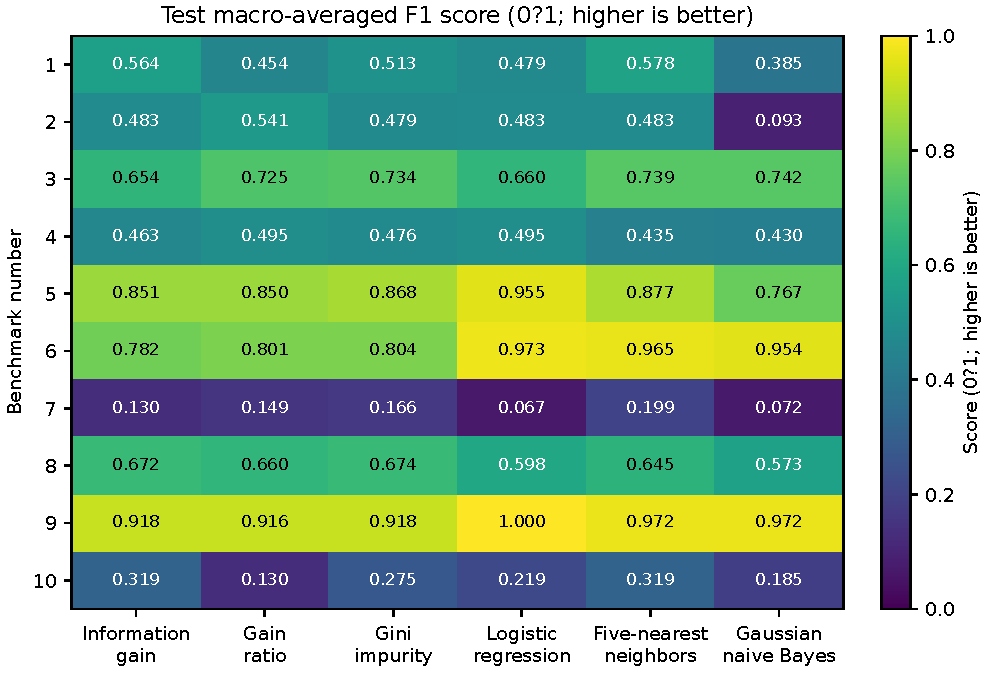
\includegraphics[width=0.95\linewidth]{figures/f1.pdf}
\caption{Macro-averaged F1 score (0--1; higher is better) across all datasets. The contrast with accuracy exposes poor
minority-class performance on Cervical Cancer and Poker.}
\label{fig:f1}
\end{figure}

\begin{table}[htbp]\centering\small
\begin{tabular}{@{}lrrrr@{}}
\toprule
Model & Accuracy (\%) & \shortstack{Macro-averaged\\F1 score (0--1)} & \shortstack{Total training\\(seconds)} & \shortstack{Total prediction\\(seconds)} \\
\midrule
Five-nearest neighbors & 75.03 & 0.6213 & 0.183 & 97.120 \\
Logistic regression & 74.82 & 0.5931 & 2.078 & 0.192 \\
Gini impurity & 73.53 & 0.5908 & 23.763 & 1.953 \\
Information gain & 73.14 & 0.5836 & 23.302 & 3.356 \\
Gain ratio & 72.40 & 0.5722 & 24.531 & 1.161 \\
Gaussian naive Bayes & 57.40 & 0.5172 & 0.162 & 0.525 \\
\bottomrule
\end{tabular}

\caption{Equal-dataset averages and sums of per-dataset mean times. Accuracy: percent correct; F1 score: 0--1 (higher is better); time: seconds (lower is faster). These aggregate
scores do not imply that one model is best on every dataset.}
\label{tab:overall}
\end{table}

Five-nearest neighbors has the highest mean accuracy and macro-averaged F1 score across these ten prepared tasks.
Logistic regression has nearly the same mean accuracy and much lower prediction time. Among tree
criteria, Gini has the highest mean scores, followed by information gain and then gain ratio. Gaussian naive Bayes has
the lowest average accuracy, but that aggregate conceals strong results on
some individual datasets. The pattern supports comparing several methods rather
than assuming that a single induction rule is universally preferable.

\subsection{Dataset-specific interpretation}
\textbf{Breast Cancer and Contraceptive Method Choice.}
Five-nearest neighbors leads Benchmark 1 with 71.93\% accuracy and macro-averaged F1 score 0.5778; its advantage over the
70.18\% training-majority accuracy is modest on only 57 test rows. On Benchmark 4, logistic regression
has the highest observed accuracy (52.54\%) and macro-averaged F1 score (0.4953), only narrowly
above gain ratio's macro-averaged F1 score of 0.4950. 

\textbf{Computer Hardware.}
Gini gives the highest accuracy (80.49\%), while Gaussian naive Bayes has the highest macro-averaged F1 score
(0.7417). Different winners under the two metrics reflect the differing weights
given to common and less common performance classes. Conclusions concern the four
chosen bands, not continuous performance prediction.

\textbf{Human Activity Recognition and Japanese Vowels.}
Logistic regression is strongest on both: 95.55\% accuracy and 0.9553 macro-averaged F1 score on Human Activity Recognition; 97.57\%
accuracy and 0.9733 macro-averaged F1 score on Vowels. The Gini tree reaches 87.07\% accuracy
on Human Activity Recognition, while the best tree accuracy on Vowels is gain ratio's 80.27\%. These observations
show that axis-aligned trees with the selected depth limit do not best exploit
every numeric representation. They do not identify whether additional depth,
pruning, feature engineering or another split geometry would close the gap.

\textbf{Poker.}
Gain ratio has the highest accuracy (57.91\%), compared with training-majority accuracy
50.12\%. Five-nearest neighbors has the highest macro-averaged F1 score (0.1992) but only 48.47\% accuracy. Even the
best macro-averaged F1 score is low, so high test-set size must not be mistaken for strong
classification performance. Fixed card positions and numeric ranks do not
explicitly encode the permutation-invariant relationships defining poker hands.
That representation is a plausible contributing limitation, not an experimentally
isolated explanation.

\textbf{Steel Industry.}
Gini gives the highest accuracy (75.78\%) and macro-averaged F1 score (0.6744). Information gain is close at
75.66\% and 0.6723. Because the training rows precede the testing rows, changes over time may
contribute to the gap between training and test accuracy. No
separate drift analysis was conducted, and same-time usage features mean the
task should not be presented as future-load forecasting.

\textbf{Wine and Wine Quality.}
Logistic regression correctly classifies all 36 Wine test rows. Five-nearest neighbors and Gaussian naive Bayes each achieve 97.22\%,
and all three trees achieve 91.67\%.  On Wine Quality, information gain has the highest accuracy (57.46\%);
five-nearest neighbors has a slightly higher macro-averaged F1 score (0.3193 versus information gain's 0.3192). Gain ratio's 43.62\%
accuracy matches the training-majority reference after rounding. The raw integer
quality labels are not merged, so this is a difficult imbalanced seven-class task.

\subsection{Why accuracy alone is insufficient: Cervical Cancer}
The test set contains 161 negative and 11 positive Biopsy labels. Information gain, logistic regression and
five-nearest neighbors all predict the negative class for every test example, giving 93.60\%
accuracy but zero positive recall. Their macro-averaged F1 score is only 0.4835. Gain ratio finds one
positive example, with four false positives, producing a higher macro-averaged F1 score of
0.5412 despite lower accuracy. Gaussian naive Bayes takes the opposite extreme: nine true positives
but 154 false positives, yielding only 9.30\% accuracy. Table~\ref{tab:cervical}
makes the errors explicit; these are benchmark results, not clinical validation.

\begin{table}[htbp]\centering\small
\begin{tabular}{@{}>{\raggedright\arraybackslash}p{1.05in}rrrrrr@{}}
\toprule
Model & \shortstack{True\\negatives} & \shortstack{False\\positives} & \shortstack{False\\negatives} & \shortstack{True\\positives} & \shortstack{Positive\\recall (0--1)} & \shortstack{Macro-averaged\\F1 score (0--1)} \\
\midrule
Information gain & 161 & 0 & 11 & 0 & 0.0000 & 0.4835 \\
Gain ratio & 157 & 4 & 10 & 1 & 0.0909 & 0.5412 \\
Gini impurity & 158 & 3 & 11 & 0 & 0.0000 & 0.4788 \\
Logistic regression & 161 & 0 & 11 & 0 & 0.0000 & 0.4835 \\
Five-nearest neighbors & 161 & 0 & 11 & 0 & 0.0000 & 0.4835 \\
Gaussian naive Bayes & 7 & 154 & 2 & 9 & 0.8182 & 0.0929 \\
\bottomrule
\end{tabular}

\caption{Benchmark 2 confusion counts (number of cases), positive recall and F1 score (0--1; higher is better). Positive means Biopsy class 1.
The columns distinguish correctly predicted negative and positive cases from false alarms and missed positive cases.}
\label{tab:cervical}
\end{table}

\subsection{Tree size and training/test gaps}
\begin{table}[htbp]\centering\scriptsize
\begin{tabular}{@{}llrrrr@{}}
\toprule
Benchmark & Split criterion & Nodes & Depth & \shortstack{Training\\accuracy (\%)} & \shortstack{Testing\\accuracy (\%)} \\
\midrule
1 & Information gain & 101 & 12 & 88.2 & 70.2 \\
1 & Gain ratio & 59 & 12 & 85.2 & 68.4 \\
1 & Gini impurity & 101 & 12 & 89.5 & 66.7 \\
2 & Information gain & 73 & 12 & 95.9 & 93.6 \\
2 & Gain ratio & 57 & 12 & 95.2 & 91.9 \\
2 & Gini impurity & 77 & 12 & 95.3 & 91.9 \\
3 & Information gain & 65 & 7 & 92.3 & 73.2 \\
3 & Gain ratio & 61 & 12 & 92.9 & 78.0 \\
3 & Gini impurity & 67 & 9 & 93.5 & 80.5 \\
4 & Information gain & 513 & 12 & 77.8 & 50.5 \\
4 & Gain ratio & 153 & 12 & 60.8 & 51.9 \\
4 & Gini impurity & 521 & 12 & 78.1 & 50.5 \\
5 & Information gain & 255 & 12 & 99.5 & 85.4 \\
5 & Gain ratio & 115 & 12 & 94.5 & 85.4 \\
5 & Gini impurity & 265 & 12 & 99.2 & 87.1 \\
6 & Information gain & 51 & 6 & 95.9 & 78.4 \\
6 & Gain ratio & 49 & 10 & 97.8 & 80.3 \\
6 & Gini impurity & 51 & 8 & 97.0 & 80.0 \\
7 & Information gain & 3427 & 12 & 67.1 & 55.4 \\
7 & Gain ratio & 1003 & 12 & 60.5 & 57.9 \\
7 & Gini impurity & 1831 & 12 & 62.5 & 54.9 \\
8 & Information gain & 693 & 12 & 94.5 & 75.7 \\
8 & Gain ratio & 303 & 12 & 92.2 & 74.9 \\
8 & Gini impurity & 741 & 12 & 95.0 & 75.8 \\
9 & Information gain & 13 & 3 & 98.6 & 91.7 \\
9 & Gain ratio & 11 & 3 & 99.3 & 91.7 \\
9 & Gini impurity & 15 & 4 & 99.3 & 91.7 \\
10 & Information gain & 1393 & 12 & 80.3 & 57.5 \\
10 & Gain ratio & 41 & 12 & 44.3 & 43.6 \\
10 & Gini impurity & 1219 & 12 & 79.8 & 56.3 \\
\bottomrule
\end{tabular}

\caption{Tree size: number of nodes; depth: maximum splits from root to leaf; training and testing: accuracy (percent correct). Metrics
are from repetition one; the deterministic tree configurations use fixed data.}
\label{tab:trees}
\end{table}
The trees often attain much higher training accuracy than test accuracy. On Human Activity Recognition,
information gain obtains 99.46\% training versus 85.41\% test accuracy. On Steel, Gini obtains
94.96\% versus 75.78\%. These gaps are consistent with limited generalization,
although the chronological Steel split can also involve distribution differences.

Gain ratio tends to produce smaller trees in several datasets, but smaller is not always
better. On Poker it uses 1,003 nodes versus information gain's 3,427 and obtains higher accuracy.
On Wine Quality it produces only 41 nodes, with training accuracy 44.26\% and
test accuracy 43.62\%, indicating little improvement even on the training set.
The direct ratio criterion, strictly positive-gain rule and depth/leaf constraints
can favor different growth patterns. The study did not test the effect of each setting separately. Future pruning and training-only tuning would be appropriate before
concluding that one criterion is intrinsically inferior.

\section{Execution time and memory}
\subsection{Training and prediction tradeoffs}
Figure~\ref{fig:times} shows per-dataset mean times on logarithmic axes, while
Appendix~\ref{sec:fullresources} provides all measurements with sample standard deviation.
The custom tree training workload is largest on Human Activity Recognition, which has 561 predictors:
mean times are approximately 10.17 seconds for information gain, 13.32 for gain ratio and 11.29 for
Gini. Poker has more training rows but only 30 encoded predictors; tree fit
times there are approximately 2.56, 1.22 and 1.39 seconds, respectively. This
illustrates why row count alone does not determine induction cost.

\begin{figure}[htbp]\centering
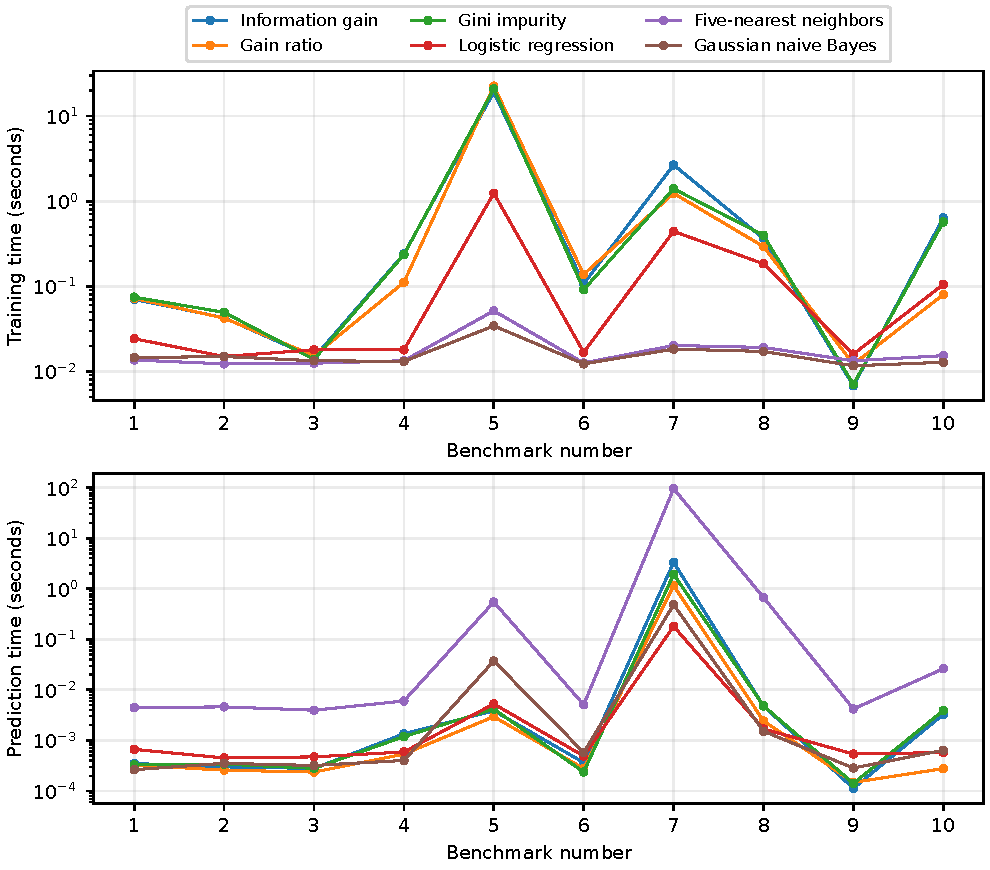
\includegraphics[width=0.97\linewidth]{figures/times.pdf}
\caption{Mean training and prediction time over three fresh-process repetitions.
Lines connect discrete datasets only to identify methods; they do not represent
an interpolation or a common dataset-size axis.}
\label{fig:times}
\end{figure}

The low training time of five-nearest neighbors reflects storing training examples rather than learning a
compact decision rule. Its Poker prediction times are 95.60, 94.49 and 93.26
seconds, averaging about 94.45 seconds. Logistic regression predicts that same test set in about
0.18 seconds on average, while the trees take approximately 1.08--3.24 seconds.
Checking distances to all training examples accounts for most of its prediction time.
All these results include the common 2,048-row batching policy, which introduces
overhead and therefore differs from the earlier unbatched pilot timings.

Gaussian naive Bayes and logistic regression benefit from compact fitted parameters and optimized library routines.
The custom tree's repeated feature sorting and count-array construction produce
substantial training work. Consequently, timings compare these implementations
as delivered, not isolated algorithmic complexity with identical low-level code.
Some fit times on small datasets are only milliseconds; their relative ordering
can reflect fixed overhead and operating-system activity as much as model work.

\subsection{Interpreting process memory}
\begin{figure}[htbp]\centering
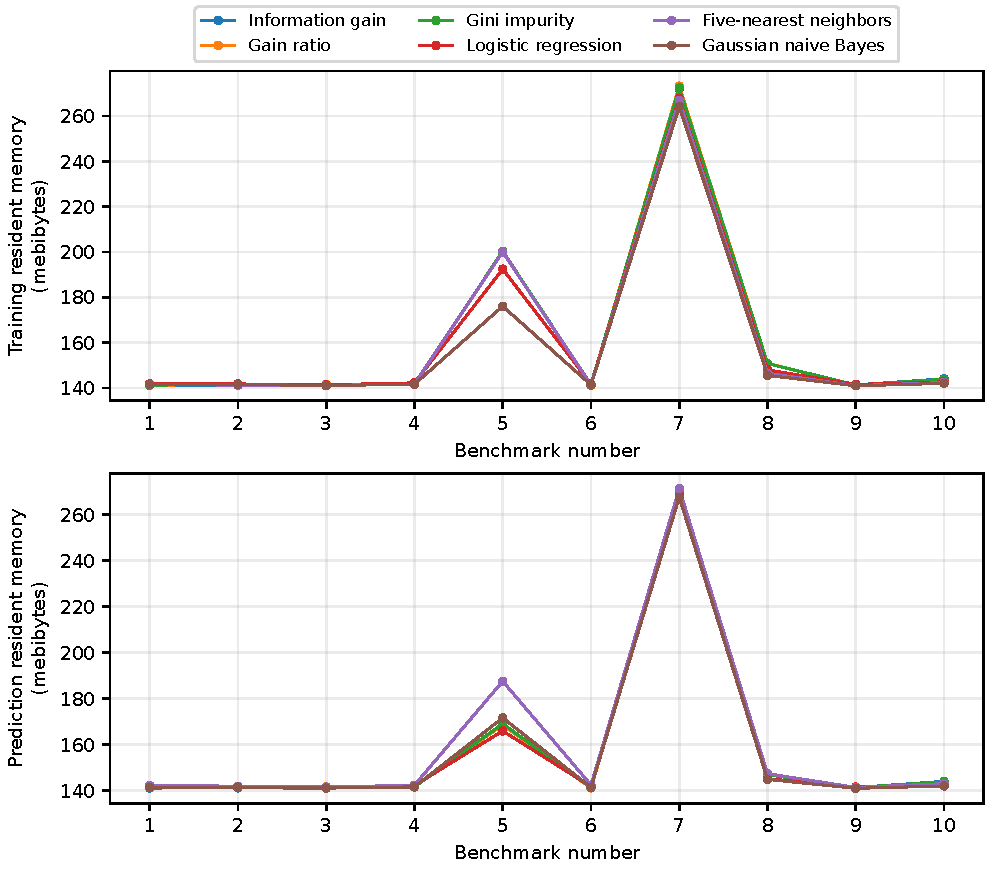
\includegraphics[width=0.97\linewidth]{figures/memory.pdf}
\caption{Mean sampled resident process memory during fit and prediction. This includes
both loaded data partitions, imported libraries and runtime state; it is not
model-only memory. Error statistics appear in Appendix~\ref{sec:fullresources}.}
\label{fig:memory}
\end{figure}

Small datasets have process peaks near 140--144 mebibytes, much of which is the common
runtime/library footprint. Human Activity Recognition's training peaks are higher because of the wide
feature matrices and training temporaries. Poker reaches roughly 263--273 mebibytes
depending on method and phase, even for algorithms with small fitted models,
because its one-million-row test matrix is already loaded during fitting.
Thus, high Poker training resident process memory does not mean that all of that memory is needed
to represent the trained classifier.

Batching limits the number of queries processed together; the code does not
allocate a single full million-by-25,010 distance matrix. It does still load
the complete test feature matrix. The measured peaks therefore describe this
in-memory evaluation design, not a streaming-data lower bound. Differences of
fractions of a mebibyte should not be overinterpreted when sampling every 5 ms.
The file \code{results/comparison/runs.csv} also records memory usage before
each phase and the increase above that starting value.

\section{Limitations and conclusions}
The validation demonstrates agreement with worked calculations, deterministic
tree behavior on small examples, and consistency of the large-run results with
saved predictions. It supports the correctness of the implemented operations;
it does not prove that every unseen input is handled correctly or that the
greedy tree is globally optimal.

The main experimental limitations are the single split per dataset, fixed
untuned hyperparameters, no pruning, retained duplicate rows, sampled rather
than exact peak memory, and differences between optimized library code and the
custom Python/NumPy implementation. Repeating the same split measures timing
variation; additional independent splits or properly nested validation would be
needed to assess how well the results generalize and to select model settings.
No statistical significance tests were performed, so small score differences
should not be treated as evidence that one classifier is reliably better.
Likewise, perfect accuracy on a small test set does not guarantee perfect
predictions on new data. Any future tuning
must refit preprocessing inside training folds and leave test data untouched.
The Hardware target adaptation, Vowels summarization, and Steel target definition
also prevent direct comparison with publications using different formulations.

Within these constraints, five-nearest neighbors achieved the best average scores but a large
prediction-time cost. Logistic regression offered nearly the same average accuracy with much
lower prediction time. Gini was the strongest custom tree configuration on
average, while individual datasets favored other criteria. The most informative
comparison is therefore the joint view of macro-averaged F1 score, accuracy, class-level errors,
training/test gaps, runtime and memory, rather than a single overall ranking.

\section{Artificial intelligence usage}
I used OpenAI Codex to assist programming and creating the algorithms. 
It assisted heavily making the processing algorithms for the ten different
benchmarks. It also reviewed my project to make sure it followed the assignment
requirements and make suggestions based on what should be included. 

The artificial intelligence assistance included:
\begin{itemize}
\item Suggesting the project structure, preprocessing approaches, and comparison
classifiers.
\item Generating and revising portions of the preprocessing, decision-tree,
comparison, evaluation, and resource-measurement code, along with tests,
comments, and documentation.
\item Helping run experiments and produce tables and figures from the saved
results, and offering explanations to support result interpretation.
\item Drafting and editing report text in LaTeX, preparing the worked example,
and helping explain the split calculations and improve presentation.
\end{itemize}


\clearpage
\appendix
\section{Complete resource measurements}\label{sec:fullresources}
The following table reports each of the 60 configurations, not just selected
winners. Values are rounded for presentation; unrounded per-repetition values
remain in \code{results/comparison/runs.csv}. A printed standard deviation of zero can mean
variation below the displayed precision. \begingroup\scriptsize\setlength{\tabcolsep}{4pt}
\begin{longtable}{@{}l>{\raggedright\arraybackslash}p{1.05in}rrrr@{}}
\caption{Resource measurements for every configuration. Each entry is mean $\pm$ sample standard deviation across three repetitions. Memory is total sampled resident process memory, not model-only memory.}\label{tab:resources}\\
\toprule Benchmark & Model & \shortstack{Training\\(seconds)} & \shortstack{Prediction\\(seconds)} & \shortstack{Training peak\\(mebibytes)} & \shortstack{Prediction peak\\(mebibytes)} \\ \midrule
\endfirsthead
\toprule Benchmark & Model & \shortstack{Training\\(seconds)} & \shortstack{Prediction\\(seconds)} & \shortstack{Training peak\\(mebibytes)} & \shortstack{Prediction peak\\(mebibytes)} \\ \midrule
\endhead
\midrule \multicolumn{6}{r}{Continued on next page}\\ \endfoot
\bottomrule \endlastfoot
1 & Information gain & $0.0701 \pm 0.0009$ & $0.0003 \pm 0.0000$ & $141.1 \pm 0.4$ & $141.1 \pm 0.4$ \\
1 & Gain ratio & $0.0722 \pm 0.0072$ & $0.0003 \pm 0.0002$ & $141.2 \pm 0.2$ & $141.2 \pm 0.2$ \\
1 & Gini impurity & $0.0745 \pm 0.0041$ & $0.0003 \pm 0.0000$ & $141.3 \pm 0.1$ & $141.3 \pm 0.1$ \\
1 & Logistic regression & $0.0242 \pm 0.0104$ & $0.0007 \pm 0.0002$ & $141.8 \pm 0.1$ & $141.8 \pm 0.1$ \\
1 & Five-nearest neighbors & $0.0136 \pm 0.0026$ & $0.0044 \pm 0.0012$ & $141.6 \pm 0.2$ & $142.3 \pm 0.2$ \\
1 & Gaussian naive Bayes & $0.0145 \pm 0.0028$ & $0.0003 \pm 0.0000$ & $141.4 \pm 0.2$ & $141.4 \pm 0.2$ \\
\addlinespace
2 & Information gain & $0.0426 \pm 0.0017$ & $0.0003 \pm 0.0000$ & $141.2 \pm 0.3$ & $141.2 \pm 0.3$ \\
2 & Gain ratio & $0.0423 \pm 0.0025$ & $0.0003 \pm 0.0000$ & $141.5 \pm 0.1$ & $141.5 \pm 0.1$ \\
2 & Gini impurity & $0.0493 \pm 0.0068$ & $0.0003 \pm 0.0000$ & $141.4 \pm 0.1$ & $141.5 \pm 0.1$ \\
2 & Logistic regression & $0.0150 \pm 0.0007$ & $0.0004 \pm 0.0000$ & $141.7 \pm 0.2$ & $141.7 \pm 0.2$ \\
2 & Five-nearest neighbors & $0.0122 \pm 0.0003$ & $0.0046 \pm 0.0001$ & $141.2 \pm 0.1$ & $141.9 \pm 0.1$ \\
2 & Gaussian naive Bayes & $0.0149 \pm 0.0029$ & $0.0004 \pm 0.0001$ & $141.5 \pm 0.1$ & $141.5 \pm 0.1$ \\
\addlinespace
3 & Information gain & $0.0145 \pm 0.0008$ & $0.0003 \pm 0.0001$ & $141.1 \pm 0.2$ & $141.1 \pm 0.2$ \\
3 & Gain ratio & $0.0152 \pm 0.0008$ & $0.0002 \pm 0.0000$ & $141.6 \pm 0.3$ & $141.6 \pm 0.3$ \\
3 & Gini impurity & $0.0138 \pm 0.0014$ & $0.0003 \pm 0.0000$ & $141.2 \pm 0.3$ & $141.2 \pm 0.3$ \\
3 & Logistic regression & $0.0179 \pm 0.0022$ & $0.0005 \pm 0.0001$ & $141.4 \pm 0.2$ & $141.4 \pm 0.2$ \\
3 & Five-nearest neighbors & $0.0125 \pm 0.0006$ & $0.0039 \pm 0.0001$ & $141.1 \pm 0.4$ & $141.5 \pm 0.4$ \\
3 & Gaussian naive Bayes & $0.0133 \pm 0.0017$ & $0.0003 \pm 0.0000$ & $141.0 \pm 0.2$ & $141.1 \pm 0.2$ \\
\addlinespace
4 & Information gain & $0.2397 \pm 0.0082$ & $0.0013 \pm 0.0002$ & $141.9 \pm 0.2$ & $141.9 \pm 0.2$ \\
4 & Gain ratio & $0.1110 \pm 0.0020$ & $0.0005 \pm 0.0000$ & $141.8 \pm 0.2$ & $141.8 \pm 0.2$ \\
4 & Gini impurity & $0.2354 \pm 0.0031$ & $0.0012 \pm 0.0000$ & $141.7 \pm 0.4$ & $141.7 \pm 0.4$ \\
4 & Logistic regression & $0.0178 \pm 0.0002$ & $0.0006 \pm 0.0001$ & $142.2 \pm 0.2$ & $142.2 \pm 0.2$ \\
4 & Five-nearest neighbors & $0.0133 \pm 0.0003$ & $0.0060 \pm 0.0003$ & $141.6 \pm 0.2$ & $142.4 \pm 0.1$ \\
4 & Gaussian naive Bayes & $0.0131 \pm 0.0012$ & $0.0004 \pm 0.0002$ & $141.6 \pm 0.2$ & $141.6 \pm 0.2$ \\
\addlinespace
5 & Information gain & $19.1524 \pm 7.5711$ & $0.0039 \pm 0.0011$ & $200.2 \pm 0.5$ & $168.7 \pm 0.5$ \\
5 & Gain ratio & $22.5292 \pm 8.3117$ & $0.0029 \pm 0.0008$ & $200.0 \pm 0.1$ & $168.5 \pm 0.1$ \\
5 & Gini impurity & $20.9246 \pm 7.2863$ & $0.0042 \pm 0.0015$ & $200.4 \pm 0.1$ & $169.1 \pm 0.1$ \\
5 & Logistic regression & $1.2401 \pm 0.0422$ & $0.0053 \pm 0.0006$ & $192.4 \pm 9.8$ & $166.0 \pm 0.2$ \\
5 & Five-nearest neighbors & $0.0514 \pm 0.0012$ & $0.5477 \pm 0.0057$ & $200.1 \pm 0.2$ & $187.6 \pm 0.2$ \\
5 & Gaussian naive Bayes & $0.0342 \pm 0.0024$ & $0.0373 \pm 0.0023$ & $176.1 \pm 7.8$ & $171.6 \pm 1.3$ \\
\addlinespace
6 & Information gain & $0.1069 \pm 0.0114$ & $0.0004 \pm 0.0002$ & $141.5 \pm 0.2$ & $141.5 \pm 0.2$ \\
6 & Gain ratio & $0.1379 \pm 0.0130$ & $0.0003 \pm 0.0000$ & $141.2 \pm 0.1$ & $141.2 \pm 0.1$ \\
6 & Gini impurity & $0.0912 \pm 0.0020$ & $0.0002 \pm 0.0000$ & $141.2 \pm 0.0$ & $141.3 \pm 0.0$ \\
6 & Logistic regression & $0.0167 \pm 0.0005$ & $0.0005 \pm 0.0000$ & $141.7 \pm 0.2$ & $141.7 \pm 0.2$ \\
6 & Five-nearest neighbors & $0.0125 \pm 0.0003$ & $0.0051 \pm 0.0010$ & $141.3 \pm 0.1$ & $142.4 \pm 0.1$ \\
6 & Gaussian naive Bayes & $0.0122 \pm 0.0003$ & $0.0006 \pm 0.0000$ & $141.3 \pm 0.1$ & $141.4 \pm 0.1$ \\
\addlinespace
7 & Information gain & $2.6687 \pm 0.0773$ & $3.3419 \pm 0.0767$ & $272.2 \pm 0.4$ & $269.4 \pm 1.0$ \\
7 & Gain ratio & $1.2387 \pm 0.0552$ & $1.1533 \pm 0.0115$ & $273.2 \pm 0.1$ & $269.4 \pm 0.6$ \\
7 & Gini impurity & $1.4001 \pm 0.0173$ & $1.9376 \pm 0.1084$ & $272.4 \pm 0.3$ & $269.2 \pm 0.3$ \\
7 & Logistic regression & $0.4418 \pm 0.0137$ & $0.1808 \pm 0.0129$ & $267.9 \pm 0.1$ & $268.7 \pm 0.7$ \\
7 & Five-nearest neighbors & $0.0201 \pm 0.0012$ & $95.8470 \pm 1.1096$ & $267.0 \pm 0.2$ & $271.3 \pm 0.2$ \\
7 & Gaussian naive Bayes & $0.0182 \pm 0.0016$ & $0.4829 \pm 0.0004$ & $264.1 \pm 0.7$ & $267.6 \pm 0.0$ \\
\addlinespace
8 & Information gain & $0.3642 \pm 0.0061$ & $0.0048 \pm 0.0004$ & $150.8 \pm 0.3$ & $147.0 \pm 0.3$ \\
8 & Gain ratio & $0.2926 \pm 0.0116$ & $0.0024 \pm 0.0004$ & $150.8 \pm 0.2$ & $147.0 \pm 0.2$ \\
8 & Gini impurity & $0.3972 \pm 0.0237$ & $0.0048 \pm 0.0001$ & $150.8 \pm 0.2$ & $147.0 \pm 0.2$ \\
8 & Logistic regression & $0.1835 \pm 0.0325$ & $0.0017 \pm 0.0003$ & $148.0 \pm 0.9$ & $145.2 \pm 0.2$ \\
8 & Five-nearest neighbors & $0.0191 \pm 0.0012$ & $0.6710 \pm 0.0080$ & $146.4 \pm 0.3$ & $147.4 \pm 0.3$ \\
8 & Gaussian naive Bayes & $0.0171 \pm 0.0012$ & $0.0015 \pm 0.0000$ & $145.5 \pm 1.0$ & $144.9 \pm 1.1$ \\
\addlinespace
9 & Information gain & $0.0068 \pm 0.0006$ & $0.0001 \pm 0.0000$ & $141.3 \pm 0.2$ & $141.3 \pm 0.2$ \\
9 & Gain ratio & $0.0121 \pm 0.0046$ & $0.0001 \pm 0.0001$ & $141.2 \pm 0.3$ & $141.2 \pm 0.3$ \\
9 & Gini impurity & $0.0070 \pm 0.0003$ & $0.0001 \pm 0.0000$ & $141.2 \pm 0.1$ & $141.3 \pm 0.1$ \\
9 & Logistic regression & $0.0159 \pm 0.0010$ & $0.0005 \pm 0.0000$ & $141.5 \pm 0.3$ & $141.6 \pm 0.2$ \\
9 & Five-nearest neighbors & $0.0133 \pm 0.0011$ & $0.0042 \pm 0.0007$ & $141.0 \pm 0.1$ & $141.4 \pm 0.1$ \\
9 & Gaussian naive Bayes & $0.0116 \pm 0.0008$ & $0.0003 \pm 0.0000$ & $140.9 \pm 0.3$ & $141.0 \pm 0.3$ \\
\addlinespace
10 & Information gain & $0.6364 \pm 0.0257$ & $0.0033 \pm 0.0000$ & $144.0 \pm 0.4$ & $144.0 \pm 0.4$ \\
10 & Gain ratio & $0.0796 \pm 0.0018$ & $0.0003 \pm 0.0000$ & $143.6 \pm 0.3$ & $143.6 \pm 0.3$ \\
10 & Gini impurity & $0.5702 \pm 0.0057$ & $0.0039 \pm 0.0007$ & $143.9 \pm 0.2$ & $143.9 \pm 0.2$ \\
10 & Logistic regression & $0.1052 \pm 0.0020$ & $0.0006 \pm 0.0000$ & $142.7 \pm 0.3$ & $142.7 \pm 0.2$ \\
10 & Five-nearest neighbors & $0.0153 \pm 0.0035$ & $0.0262 \pm 0.0006$ & $142.4 \pm 0.2$ & $143.0 \pm 0.3$ \\
10 & Gaussian naive Bayes & $0.0128 \pm 0.0010$ & $0.0006 \pm 0.0000$ & $142.0 \pm 0.1$ & $142.0 \pm 0.1$ \\
\addlinespace
\end{longtable}

\endgroup

\end{document}
